

\subsection{Covid nowcasting} \label{sec:application-covid}

During the COVID-19 pandemic, the need for reliable and timely nowcasts of the pandemic's development has become apparent.
In Germany, the seven-day hospitalization rate was established as a central steering measure for COVID-19 measures in November 2021, and the imposition of severe public restrictions was based on it~\parencite{RobertKochInstitute2021}.
The Robert Koch Institute (RKI) provides daily reports on the number of new hospitalizations.
However, these reports are subject to delays and revisions in two sources.
The first source is technical delays in the reporting process, for example, due to different authorities passing the data to the RKI~\parencite{RobertKochInstitute2024}.
The second, more systematic source is the structure of the seven-day hospitalization rate.
To a given date, all the cases are allocated whose first positive test result was on that date and who were hospitalized in relation to the disease in the following.
The seven-day hospitalization rate is the average count of cases per $100,000$ inhabitants on the given date and six days before.
Thus, the final seven-day hospitalization rate can only be reported with a significant delay of up to more than 70 days.
Nevertheless, as the seven-day hospitalization rate was considered a major indicator of the pandemic's development, many organizations and institutions started to issue nowcasts, including research teams and newspapers.
To collect nowcasts of the seven-day hospitalization rate by different nowcast groups, the COVID19-Nowcasting-Hub was established~\parencite{ChairOfEconometricsAndStatisticsAtKarlsruheInstituteOfTechnology2024}.
The nowcasts contain the seven-day hospitalization rate's predictive mean, median, and quantiles.
\unsure{median ist ja auch quantile}
\begin{figure}
    \centering
    \begin{subfigure}[t]{0.48\textwidth}
    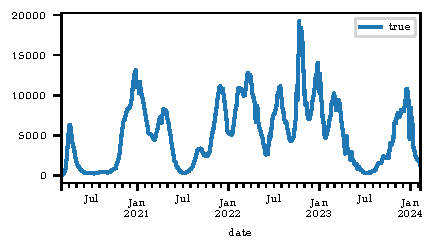
\includegraphics{plots/covid_nowcast/00_true_data.pdf}
    \caption{Realisations.}
    \label{fig:app-covid-true}
    \end{subfigure}\hfill
    \begin{subfigure}[t]{0.48\textwidth}
    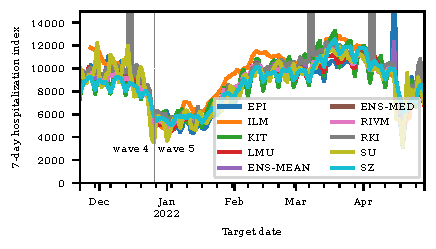
\includegraphics{plots/covid_nowcast/00_nowcast_data.pdf}
    \caption{Same-day nowcasts}
    \label{fig:app-covid-nowcast}
        \end{subfigure}
    \caption{True and nowcast data of the seven-day-hospitalization in Germany from November 22, 2021, to April 29, 2022 \parencite{ChairOfEconometricsAndStatisticsAtKarlsruheInstituteOfTechnology2024}.
    The outliers in the RKI model of values above $10^8$ are removed before the following analysis.}
    \label{fig:app-covid-true-nowcast}
\end{figure}


The data contains eight nowcasts from scientific and public institutions, nowcast communities, and a newspaper, using different input variables, calendar data, and length of training data.
The model structures are diverse, including Bayesian models, generalized additive models, and parametric bootstrapping.
Table~\ref{tab:app-covid-models} in the appendix lists the different abbreviations and the model's overall structure.
Using the nowcasts, two ensemble methods are constructed using the ensembles' mean or median.
We denote them by ENS-MEAN and ENS-MED.
In line with the initial study design, we consider the period from November 22, 2021, to April 29, 2022, as the evaluation period.
In contrast to~\textcite{Wolffram2023}, we use the newest data available on the true values, not the data from August 8, 2022.
\unsure{Nochmal längere Evaluation?}
We do not expand on the models' performance on specific regions or age groups in Germany and the probabilistic nowcast assessment.
Figure~\ref{fig:app-covid-true-nowcast} displays the true and nowcast data for the evaluation period.
The time comprises the fourth wave's end in December 2021 and nearly the entire fifth wave of the pandemic in Germany, lasting until May 28, 2022~\parencite{Tolksdorf2022}.
Table~\ref{tab:app-covid-rmse} summarizes the point evaluation measures for the issued mean of the different models.
The models issue same-day nowcasts for nearly all 159 days of the evaluation period~\parencite[see][Tables A2, A3, and A4]{Wolffram2023}.
The best-performing models in terms of RMSE and MAE are the ILM and RKI models.
The ensemble methods perform worse than the best models regarding the mean location.
The performance of the models is diverse, with more than twice as high RMSE values for the worst models compared to the best models.
Note that the high values for the EPI model could be driven by an exceptionally far-off value at the end of the evaluation period.

In addition to close inspection of the point evaluation measures, assessing the trending of the nowcasts is crucial.
To assess the impact of taken measures and the direction of the curve, it is essential to distinguish between rising and falling hospitalization rates.
If hospitalization rates rise, measures should be tightened, while falling rates might allow for loosening measures.
Especially, asymmetries are of interest to assess whether some models are better at recognizing a fall than a rise or vice versa.

\begin{table}[]
    \centering
    \begin{tabular}{llllr}
\toprule
 & rmse & mae & mse & count \\
model &  &  &  &  \\
\midrule
ILM-prop & :,.f & :,.f & :,.f & 530 \\
RIVM-KEW & :,.f & :,.f & :,.f & 817 \\
NowcastHub-MeanEnsemble & :,.f & :,.f & :,.f & 610 \\
NowcastHub-MedianEnsemble & :,.f & :,.f & :,.f & 610 \\
LMU_StaBLab-GAM_nowcast & :,.f & :,.f & :,.f & 574 \\
RKI-weekly_report & :,.f & :,.f & :,.f & 334 \\
KIT-simple_nowcast & :,.f & :,.f & :,.f & 861 \\
SZ-hosp_nowcast & :,.f & :,.f & :,.f & 535 \\
SU-hier_bayes & :,.f & :,.f & :,.f & 423 \\
Epiforecasts-independent & :,.f & :,.f & :,.f & 275 \\
\bottomrule
\end{tabular}

    \caption{Point evaluation measures for the issued mean of the different models. The evaluation period comprises 159 days. }
    \label{tab:app-covid-rmse}
\end{table}

\subsubsection*{Results}

In the following, we apply the trending assessment of Section~\ref{sec:trending} to the nowcasts of the seven-day hospitalization rate.
We report the trending for the lags 1, 7, and 14 days.
While lag 1 assesses the short-term trending, lags 7 and 14 consider the medium-term trending.
The lags 7 and 14 are particularly interesting, reflecting a usual period until new policy changes are taken.

Before stating the results, we provide background information on the marginal distributions of the true values and nowcasts for the different lags.
Table~\ref{tab:app-covid-marginals} in Appendix~\ref{sec:appendix-application-covid} provides information on marginal statistics of the nowcasts and true values.
Overall, the variability and general level of differences grow with the lag.
The standard deviation increases from roughly 300 for lag 1 to 1,200 for lag 7 and 2,000 for lag 14.
Similarly, the 10\%-quantile of differences increases.
The 10\%-quantile is used for the exclusion areas in the trending assessment.
The exclusion area is rectangular; a point falls within it if both $\diffy$ and $\diffx$ are below the respective 10\%-quantile of the differences.
Thus, points are still included in the trending assessment if they are large in one dimension but not in the other, thus ensuring that substantial changes in, e.g., $\diffy$ are to be recognized by the nowcast and vice versa.

Table~\ref{tab:app-covid-trending-ratios-lag-7} lists the trending ratios for all models with and without exclusion areas for the lag of 7 days.
The trending ratios without exclusion area range from 0.72 to 0.85 for the lag of 7 days.
The negative trending ratios are higher than the positive trending ratios for all models.
For all models, the confidence intervals for the positive and negative trending ratios do not overlap, indicating that the trending ratios are indeed different.
The 10\%-quantile exclusion areas have, at most, an influence of 0.03 on the ratios.
The model with the highest trending ratio is the ILM model, and the model with the lowest is the RKI model.
The confidence intervals between all models overlap, reflecting the evaluation period lasting 159 days.
The positive trending ratio implies a similar ranking of the models, while the negative ratio is second best for the RKI model.
For the lags of 1 and 14 days, we refer to Table~\ref{tab:app-covid-trending-ratios-lag-1-14} in Appendix~\ref{sec:appendix-application-covid}.

Figure~\ref{fig:app-covid-cond-prob-trending-ratio-7} shows the conditional trending plots and the trending ratio over the exclusion area for the lag seven days; the respective plots for the lags one day and 14 days are shown in Figure~\ref{fig:app-covid-cond-prob-trending-ratio-1-14}.
Here, only the best models in point evaluation measures, ILM, RKI, RIVM, and ENS-MED, are shown to keep the plots readable.
If RKI or ILM issues a fall in the hospitalization rate, the probability of a fall is higher than if RIVM or ENS-MED issues a fall.
The opposite is the case for a nowcasted hospitalization rate increase, and the probability margin is higher. \todo{was soll das heißen?}
Similar observations can be made for the lag of 14 days in Figure~\ref{fig:app-covid-cond-prob-14}.
For a lag of one day, the models' conditional trending ability difference is less pronounced (see Figure~\ref{fig:app-covid-cond-prob-1}).
The RKI model is still less conclusive when issuing an increase in the hospitalization rate, while RIVM is most informative in that case.
The curves cross for an issued fall, with ENS-MED being on top for issued falls above 250.

The trending ratios are plotted for various exclusion areas in Figure~\ref{fig:app-covid-trending-ratio-7}.
In general, the trending ratio increases with larger exclusion areas.
While the RIVM and ENS-MED trending ratios evolve similarly, the RKI and ILM trending ratios get closer.
For the lag of 1 day, the RKI trending ratio decreases with increasing exclusion area size while the other models evolve increasingly (see Figure~\ref{fig:app-covid-trending-ratio-1}).
For the lag of 14 days, all trending ratio curves increase with the exclusion area size (see Figure~\ref{fig:app-covid-trending-ratio-14}).

\begin{table}
    \centering
    \tiny
    \begin{tabular}{l p{0.11\textwidth} p{0.11\textwidth} p{0.11\textwidth} p{0.11\textwidth} p{0.11\textwidth} p{0.11\textwidth}}
\toprule
 & $\mu^{7}$ & $\mu^{+, 7}$ & $\mu^{-, 7}$ & $\mu^{7}_{q_{0.1}}$ & $\mu^{+, 7}_{q_{0.1}}$ & $\mu^{-, 7}_{q_{0.1}}$ \\
\midrule
EPI & {0.77\newline(0.71, 0.82)} & {0.67\newline(0.59, 0.76)} & {0.87\newline(0.79, 0.92)} & {0.78\newline(0.72, 0.83)} & {0.68\newline(0.59, 0.75)} & {0.88\newline(0.80, 0.93)} \\
ILM & {0.85\newline(0.80, 0.90)} & {0.73\newline(0.64, 0.80)} & {0.99\newline(0.94, 1.00)} & {0.85\newline(0.80, 0.90)} & {0.74\newline(0.65, 0.81)} & {0.99\newline(0.94, 1.00)} \\
KIT & {0.74\newline(0.68, 0.80)} & {0.64\newline(0.55, 0.72)} & {0.87\newline(0.80, 0.93)} & {0.75\newline(0.69, 0.80)} & {0.64\newline(0.55, 0.72)} & {0.88\newline(0.81, 0.94)} \\
LMU & {0.80\newline(0.74, 0.85)} & {0.70\newline(0.62, 0.77)} & {0.91\newline(0.84, 0.95)} & {0.81\newline(0.75, 0.86)} & {0.72\newline(0.63, 0.79)} & {0.92\newline(0.85, 0.96)} \\
ENS-MEAN & {0.82\newline(0.76, 0.86)} & {0.71\newline(0.63, 0.78)} & {0.94\newline(0.89, 0.97)} & {0.82\newline(0.76, 0.87)} & {0.71\newline(0.63, 0.78)} & {0.96\newline(0.90, 0.99)} \\
ENS-MED & {0.82\newline(0.77, 0.86)} & {0.70\newline(0.61, 0.78)} & {0.96\newline(0.90, 0.99)} & {0.83\newline(0.77, 0.87)} & {0.72\newline(0.64, 0.79)} & {0.96\newline(0.90, 0.99)} \\
RIVM & {0.83\newline(0.77, 0.87)} & {0.74\newline(0.65, 0.81)} & {0.92\newline(0.86, 0.96)} & {0.83\newline(0.78, 0.88)} & {0.74\newline(0.65, 0.81)} & {0.93\newline(0.87, 0.97)} \\
RKI & {0.72\newline(0.65, 0.77)} & {0.60\newline(0.51, 0.67)} & {0.98\newline(0.92, 1.00)} & {0.73\newline(0.66, 0.78)} & {0.61\newline(0.53, 0.68)} & {0.98\newline(0.92, 1.00)} \\
SU & {0.81\newline(0.75, 0.86)} & {0.71\newline(0.62, 0.79)} & {0.92\newline(0.85, 0.96)} & {0.81\newline(0.75, 0.85)} & {0.71\newline(0.63, 0.79)} & {0.92\newline(0.85, 0.96)} \\
SZ & {0.78\newline(0.72, 0.83)} & {0.67\newline(0.58, 0.75)} & {0.91\newline(0.84, 0.96)} & {0.78\newline(0.72, 0.83)} & {0.67\newline(0.58, 0.75)} & {0.92\newline(0.85, 0.97)} \\
\bottomrule
\end{tabular}

    \caption{The trending ratio $\accl[7]$, positive trending ratio $\accpl[l]$, and negative trending ratio $\accml[l]$ for the models with and without exclusion areas for the lag seven days. The exclusion areas are rectangles centered on the zero points with a width and height of 10\%-quantile of the absolute values of nowcast and true values. }
    \label{tab:app-covid-trending-ratios-lag-7}
\end{table}

\begin{figure}
    \centering
%    \includegraphics{}
    \begin{subfigure}[t]{.48\textwidth}
    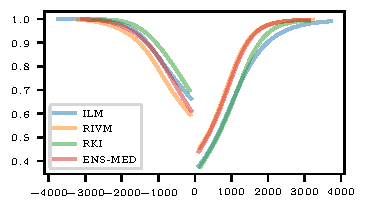
\includegraphics{plots/covid_nowcast/40_cond_prob_lag_7}
    \caption{Conditional trending plot.}\label{fig:app-covid-cond-prob-7}
    \end{subfigure}\hfill
    \begin{subfigure}[t]{.48\textwidth}
    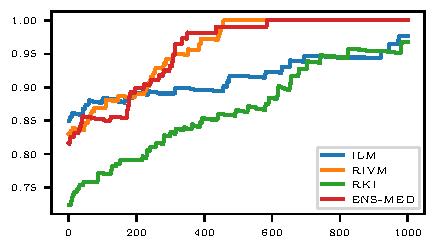
\includegraphics{plots/covid_nowcast/40_acc_eps_lag_7}
    \caption{Trending ratio over exclusion area size in $\diffx$.}\label{fig:app-covid-trending-ratio-7}
    \end{subfigure}
    \caption{Conditional trending plot and trending ratio over exclusion area for the nowcasts of the seven-day hospitalization rate ILM, RKI, RIVM, and ENS-MED for the lag seven days.}
    \label{fig:app-covid-cond-prob-trending-ratio-7}
\end{figure}



\subsubsection*{Discussion}

For all lags, the influence of the exclusion area on the 10\%-quantile level is negligible.
For example, the trending ratio changes at most by 0.03 for the EPI model with $\acc^{-, 14}$.
The exclusion areas are thus not crucial for the trending assessment in the case of the nowcasts of the seven-day hospitalization rate.
The lower bound of confidence intervals is at least 0.68 for all models, indicating that they perform better than random guessing the trend.

Trending assessment is unattached to point evaluation measures.
RKI is among the best in point evaluation measures but performs worse in trending assessment.
The assessment of asymmetry in the conditional trending plots is crucial for interpreting the trending ratios, with the RKI model being the most prominent example.

A more extensive training size would be beneficial for assessing the models' performance.
For some models, more data is accessible, but we stick with the study protocol that uses an evaluation period of 159 days.

\subsection{Forecasting emergency department arrivals}\label{sec:application-eda}

In a second example, we consider the forecasting of the hourly number of arrivals in a large emergency department.
Forecasting the number of arrivals in an emergency department is crucial for planning staff and resources.
In \textcite{Rostami-Tabar2023}, various models are employed to forecast the hourly number of arrivals in a large emergency department.
Every 12 hours, the models issue hourly forecasts for the next 48 hours.
Thus, the management can take measures according to the expected number of arrivals, for example, through redeploying staff and reconfiguring units.
The models issue probabilistic quantile forecasts, which are evaluated through RMSE, pinball loss, pinball skill scores, and PIT-histograms.
The models are trained on data from April 1, 2014, to February 28, 2018, and evaluated on data from March 1, 2018, to February 28, 2019.
For further notes on the models and the evaluation, we refer to \textcite{Rostami-Tabar2023}.
From the issued forecasts, we use the mean as a point forecast for the trending assessment.
We use the forecasts issued at the first time point for every target time.
Thus, the forecasts are issued 36 to 48 hours ahead of the target time, and the emergency department management has time to adjust the measures according to the expected number of arrivals.
Considering only the forecasts of at least 36 hours ahead, we restrict the evaluation period to March 2, 2018, at noon, to February 28, 2019, at 23:00, comprising 8,724 hours.

In this setup, trending assessment is a simple and intuitive way to assess the models' performance.
It is easy for the management to understand and implement, as simple comparisons of the expected workload to an hour in the recent past can be made.
If, for example, the staff was near capacity in the last shift and an increase in the number of arrivals is expected, the management can take measures to adjust the workload.

The number of arrivals has a strong weekly and daily pattern.
Thus, we consider the lags of 72 hours, the last already observed shift of the same hour of day, and seven days, the previous shift of the same hour and day.
Table~\ref{tab:app-eda-point-evaluation} lists the point evaluation measures for the models.
The best-performing models regarding RMSE and MAE are the NBI-2 and Poisson-2 models.
More than 8,600 forecasts are available for all models, with differences in the number due to missing values on four afternoons in 2018.
Note that the reported values for the RMSE differ from those in \textcite{Rostami-Tabar2023}.
In contrast to their work, we use only the forecast data at least 36 hours ahead and not the entire forecast data for evaluation.

\begin{table}
\centering
\begin{tabular}{l r r r}
\toprule
Model & RMSE & MAE & Count \\
\midrule
NBI-2 & 8.883 & 3.200 & 8688 \\
Poisson-2 & 8.884 & 3.200 & 8688 \\
Poisson-1 & 9.164 & 3.238 & 8688 \\
Benchmark-2 & 9.246 & 3.236 & 8688 \\
Ttr-2 & 9.394 & 3.266 & 8688 \\
NOtr-1 & 9.413 & 3.276 & 8688 \\
NOtr-2 & 9.413 & 3.276 & 8688 \\
Poisson-2-I & 9.458 & 3.276 & 8688 \\
Benchmark-1 & 10.065 & 3.331 & 8688 \\
GBM-2 & 11.663 & 3.542 & 8688 \\
tbats & 12.905 & 3.912 & 8724 \\
Prophet & 13.078 & 3.877 & 8724 \\
qreg-1 & 13.337 & 3.758 & 8688 \\
Regression-Poisson & 21.162 & 4.818 & 8724 \\
ADAM-iETSX & 28.000 & 5.561 & 8724 \\
ETS & 29.358 & 5.742 & 8724 \\
\bottomrule
\end{tabular}

\caption{Point evaluation measures for the models. The smaller count for some models stems from missing forecasts for a few hours in the course of the evaluation period.}\label{tab:app-eda-point-evaluation}
\end{table}


\subsubsection*{Results}

Table~\ref{tab:app-eda-marginals} analyzes the differences in marginal distributions for the forecasts and true values for the lags of 3 and 7 days.
Note that the difference definition aligns with Section~\ref{sec:notation}, defined as the difference between the forecasted mean and true value of 3 and 7 days before, as the true value is available when issuing the forecast.
The fraction of positive differences varies between 0.39 and 0.63 for the lag of 3 days and between 0.37 and 0.63 for the lag of 7 days.
The variability of differences decreases for the larger lag for most models; only for the ETS model does it increase.
The 10\%-quantile of the differences is between zero and one for all models and lags.
Thus, we exclude only values smaller than one from the trending assessment.
The resulting fraction of included values in the computation is also listed in Table~\ref{tab:app-eda-marginals} and is at least 79\% of the values.

\begin{table}
    \centering
    \begin{tabular}{lllllllll}
\toprule
 & (1), l=3 & $\sigma_{x^{\Delta, 3}}$ & $q_{0.1} (x^{\Delta, 3})$ & (2), l=3 & (1), l=7 & $\sigma_{x^{\Delta, 7}}$ & $q_{0.1} (x^{\Delta, 7})$ & (2), l=7 \\
\midrule
ADAM-iETSX & 0.57 & 7.76 & 0.83 & 0.88 & 0.57 & 7.49 & 0.78 & 0.87 \\
Benchmark-1 & 0.45 & 5.05 & 0.50 & 0.80 & 0.44 & 4.43 & 0.47 & 0.78 \\
Benchmark-2 & 0.51 & 5.11 & 0.52 & 0.80 & 0.50 & 4.29 & 0.45 & 0.78 \\
ETS & 0.58 & 7.49 & 0.78 & 0.87 & 0.58 & 7.68 & 0.84 & 0.88 \\
GBM-2 & 0.39 & 4.93 & 0.51 & 0.80 & 0.37 & 4.61 & 0.49 & 0.79 \\
NBI-2 & 0.53 & 5.04 & 0.52 & 0.81 & 0.53 & 4.41 & 0.48 & 0.79 \\
NOtr-1 & 0.52 & 5.03 & 0.51 & 0.81 & 0.51 & 4.41 & 0.49 & 0.79 \\
NOtr-2 & 0.52 & 5.03 & 0.51 & 0.81 & 0.51 & 4.41 & 0.49 & 0.79 \\
Poisson-1 & 0.53 & 5.04 & 0.51 & 0.81 & 0.52 & 4.38 & 0.48 & 0.79 \\
Poisson-2 & 0.53 & 5.05 & 0.52 & 0.80 & 0.53 & 4.42 & 0.48 & 0.78 \\
Poisson-2-I & 0.51 & 5.03 & 0.51 & 0.81 & 0.50 & 4.42 & 0.49 & 0.79 \\
Prophet & 0.62 & 5.27 & 1.00 & 0.91 & 0.62 & 5.15 & 1.00 & 0.91 \\
Regression-Poisson & 0.51 & 6.65 & 0.67 & 0.85 & 0.51 & 6.49 & 0.67 & 0.85 \\
Ttr-2 & 0.51 & 5.03 & 0.50 & 0.81 & 0.50 & 4.41 & 0.49 & 0.79 \\
qreg-1 & 0.39 & 5.01 & 0.49 & 0.81 & 0.39 & 4.84 & 0.51 & 0.80 \\
tbats & 0.63 & 5.35 & 1.00 & 0.92 & 0.63 & 5.04 & 1.00 & 0.92 \\
True & 0.54 & 6.61 & 1.00 & 0.93 & 0.55 & 5.90 & 1.00 & 0.92 \\
\bottomrule
\end{tabular}

    \caption{Marginal analysis of the nowcast and true differences. The column (1), $l=l$ shows the fraction of values greater than zero for lag $l$, $\sigma_{x^{\Delta, l}}$ the standard deviation, and $q_{0.1} (x^{\Delta, l})$ the 10\% quantile of the differences' absolute values.}
    \label{tab:app-eda-marginals}
\end{table}

Table~\ref{tab:app-eda-trending-ratios} lists the trending ratios for all models for three and seven-day lags.
The trending ratios range from 0.68 to 0.84 for a lag of three days and from 0.68 to 0.82 for seven days.
The negative and positive trending ratios differ for all models and lags.
For some models, for example, the GBM-2 model, the positive trending ratio is higher; for some models, for example, the tbats model, the negative trending ratio is higher.
The confidence interval width is at most 0.02 for the trending ratios and at most 0.03 for the positive and negative trending ratios.
The positive trending ratio is higher for other models than the negative trending ratio.
The models GBM-2, qreg-1, and Benchmark-1 have the highest positive trending ratio for the lag of 3 and seven days, while Poisson-2 and NBI-2 have the highest negative trending ratio.

Figure~\ref{fig:app-eda-cond-prob} shows the conditional trending plots for the models Benchmark-1, GBM-2, NBI-2, Poisson-2, and qreg-1 for the lags 3 and 7 days and thus inspects the local trending ability of the models with highest positive and negative trending ratio.
The conditional trending plots show similar courses for the two lags, while the curves are shifted downwards for the lag of seven days.
The model's relative trending ability evolves consistently for the two lags, with the NBI-2 and Poisson-2 models being indistinguishable.
The GBM-2 model outperforms the qreg-1 model for all $x$.
The models NBI-2 and Poisson-2 have the highest trending ability for all negative values of $x$ and the lowest trending ability for all positive values of $x$.
Benchmark-1 lies between the other models for all $x$.

\begin{table}
    \centering
    \begin{tabularx}{\textwidth}{X p{0.11\textwidth} p{0.11\textwidth} p{0.11\textwidth} p{0.11\textwidth} p{0.11\textwidth} p{0.11\textwidth}}
\toprule
 & $\mu^{3}$ & $\mu^{+, 3}$ & $\mu^{-, 3}$ & $\mu^{7}$ & $\mu^{+, 7}$ & $\mu^{-, 7}$ \\
\midrule
ADAM-iETSX & {0.70\newline(0.69, 0.71)} & {0.68\newline(0.67, 0.69)} & {0.72\newline(0.71, 0.73)} & {0.68\newline(0.67, 0.69)} & {0.67\newline(0.66, 0.69)} & {0.69\newline(0.67, 0.70)} \\
Benchmark-1 & {0.83\newline(0.82, 0.84)} & {0.86\newline(0.85, 0.87)} & {0.81\newline(0.79, 0.82)} & {0.81\newline(0.80, 0.82)} & {0.86\newline(0.85, 0.87)} & {0.78\newline(0.76, 0.79)} \\
Benchmark-2 & {0.84\newline(0.83, 0.84)} & {0.83\newline(0.82, 0.85)} & {0.84\newline(0.83, 0.85)} & {0.82\newline(0.81, 0.83)} & {0.83\newline(0.82, 0.84)} & {0.80\newline(0.79, 0.82)} \\
ETS & {0.68\newline(0.67, 0.69)} & {0.66\newline(0.65, 0.67)} & {0.70\newline(0.69, 0.72)} & {0.67\newline(0.66, 0.68)} & {0.66\newline(0.64, 0.67)} & {0.68\newline(0.66, 0.69)} \\
GBM-2 & {0.82\newline(0.81, 0.82)} & {0.90\newline(0.89, 0.91)} & {0.77\newline(0.76, 0.78)} & {0.78\newline(0.77, 0.79)} & {0.88\newline(0.87, 0.90)} & {0.73\newline(0.72, 0.74)} \\
NBI-2 & {0.84\newline(0.83, 0.85)} & {0.83\newline(0.82, 0.84)} & {0.85\newline(0.84, 0.86)} & {0.82\newline(0.81, 0.83)} & {0.82\newline(0.81, 0.83)} & {0.82\newline(0.81, 0.83)} \\
NOtr-1 & {0.83\newline(0.83, 0.84)} & {0.83\newline(0.82, 0.84)} & {0.84\newline(0.82, 0.85)} & {0.81\newline(0.80, 0.82)} & {0.82\newline(0.81, 0.83)} & {0.80\newline(0.79, 0.81)} \\
NOtr-2 & {0.83\newline(0.83, 0.84)} & {0.83\newline(0.82, 0.84)} & {0.84\newline(0.82, 0.85)} & {0.81\newline(0.80, 0.82)} & {0.82\newline(0.81, 0.83)} & {0.80\newline(0.79, 0.81)} \\
Poisson-1 & {0.84\newline(0.83, 0.84)} & {0.82\newline(0.81, 0.83)} & {0.85\newline(0.84, 0.86)} & {0.82\newline(0.81, 0.82)} & {0.82\newline(0.81, 0.83)} & {0.81\newline(0.80, 0.82)} \\
Poisson-2 & {0.84\newline(0.83, 0.85)} & {0.83\newline(0.82, 0.84)} & {0.85\newline(0.84, 0.86)} & {0.82\newline(0.81, 0.82)} & {0.82\newline(0.81, 0.83)} & {0.82\newline(0.80, 0.83)} \\
Poisson-2-I & {0.83\newline(0.83, 0.84)} & {0.84\newline(0.83, 0.85)} & {0.83\newline(0.82, 0.84)} & {0.81\newline(0.80, 0.82)} & {0.83\newline(0.81, 0.84)} & {0.80\newline(0.79, 0.81)} \\
Prophet & {0.75\newline(0.74, 0.76)} & {0.72\newline(0.71, 0.73)} & {0.79\newline(0.77, 0.80)} & {0.74\newline(0.73, 0.74)} & {0.72\newline(0.70, 0.73)} & {0.76\newline(0.75, 0.77)} \\
Regression-Poisson & {0.72\newline(0.71, 0.73)} & {0.73\newline(0.71, 0.74)} & {0.72\newline(0.70, 0.73)} & {0.70\newline(0.69, 0.71)} & {0.71\newline(0.70, 0.73)} & {0.69\newline(0.67, 0.70)} \\
Ttr-2 & {0.84\newline(0.83, 0.84)} & {0.84\newline(0.83, 0.85)} & {0.83\newline(0.82, 0.85)} & {0.81\newline(0.80, 0.82)} & {0.83\newline(0.82, 0.84)} & {0.80\newline(0.79, 0.81)} \\
qreg-1 & {0.80\newline(0.79, 0.80)} & {0.88\newline(0.87, 0.89)} & {0.75\newline(0.74, 0.76)} & {0.77\newline(0.76, 0.78)} & {0.86\newline(0.85, 0.88)} & {0.71\newline(0.70, 0.72)} \\
tbats & {0.75\newline(0.74, 0.76)} & {0.72\newline(0.71, 0.73)} & {0.80\newline(0.78, 0.81)} & {0.73\newline(0.72, 0.74)} & {0.71\newline(0.69, 0.72)} & {0.76\newline(0.74, 0.77)} \\
\bottomrule
\end{tabularx}

    \caption{Trending ratio $\acc$, positive trending ratio $\accp$, and negative trending ratio $\accm$ for the models with the exclusion of zero-containing points for the lags 72 hours and seven days.}
    \label{tab:app-eda-trending-ratios}
\end{table}

\begin{figure}
    \centering
    \begin{subfigure}[t]{0.48\textwidth}
    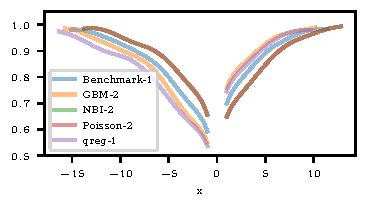
\includegraphics{plots/ed_arrival/50_Cond_Prob_lag_3}
    \caption{Lag 3 days}
    \end{subfigure}\hfill
    \begin{subfigure}[t]{0.48\textwidth}
    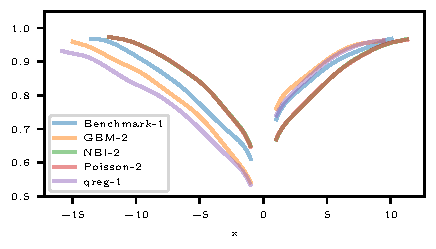
\includegraphics{plots/ed_arrival/50_Cond_Prob_lag_7}
    \caption{Lag 7 days}
    \end{subfigure}
    \caption{Conditional trending plots for the lags 3 and 7 days and the models with the best positive or negative trending ability. The plots of NBI-2 and Poisson-2 are indistinguishable.}
    \label{fig:app-eda-cond-prob}
\end{figure}

\subsubsection*{Discussion}

Trending ability is consistent for the two lags, with the models' relative trending ability evolving similarly for the two lags.
The models' trending ability is generally higher for the smaller lag, but the differences are minor, and confidence intervals overlap.

The trending differs for all models for positive and negative predicted change directions.
While some models, such as GBM-2 and qreg-1, have the highest positive trending ratio, others, such as Poisson-2 and NBI-2, have the highest negative trending ratio.
Thus, the uncertainty of the model's predicted change has to be assessed differently based on the direction.

The example shows that trending assessment is detached from standard point evaluation measures.
While the models with the lowest RMSE, NBI-2 and Poisson-2, also have a high trending ability, three models with below-average point evaluation measures, Benchmark-1, GBM-2, and qreg-1, have a high positive trending ability.


\subsection{Invasive and non-invasive blood pressure monitoring} \label{sec:application_measurement}

In the last briefer example, we consider the trending assessment of measurement data.
The data is from the MIMIC-III database, including various information on patients in critical care units of the Beth Israel Deaconess Medical Center in Boston (Massachusetts, USA, \cite{Johnson2016}).
The data is publicly available and also includes numerical measurement data such as heart rate, blood pressure, and oxygen saturation in a waveform database \parencites[][]{Moody2017}[available through][]{Goldberger2000}.

For some patients, the data includes \ac{abp} and \ac{nbp} measurements.
For an overview of blood pressure measurement methods, see \textcite{Saugel2014}.
While non-invasive blood pressure measurement methods are relatively gentle, they are less accurate than invasive methods.
For critical patients, changes in blood pressure can be crucial for the treatment.
Thus, trending assessment can be performed in addition to standard accuracy analysis~\parencite[see, e.g., ]{Mostafa2020}.
Thus, we assess the trending ability of the non-invasive blood pressure measurements compared to the invasive blood pressure measurements.
Of the 64,168 numerical data records in the database, 2,662 include at least one measurement of systolic \ac{abp} and \ac{nbp} and ... include at least measurements of \ac{abp} and \ac{nbp} at the same time.
The data records generally include measurements for one patient.

We consider the lags of one minute, five minutes, and 15 minutes for the trending assessment, as those are typical intervals of NBP measurements.
The number of available records with measurements of \ac{abp} and \ac{nbp} for the lags are listed in Table~\ref{tab:app-mimic-data-summary}.

\begin{table}
    \centering
    \caption{Data summary of the \ac{abp} and \ac{nbp} measurements for the lags one minute, five minutes, and 15 minutes.}
    \label{tab:app-mimic-data-summary}
\end{table}

\subsubsection*{Results}

Again, we exclude the 10\% of absolute differences in trending assessment.
The resulting four-quadrant plots of the mean and systolic blood pressure measurements for the different lags are shown in Figure~\ref{fig:app-mimic-4q}.
The number of points in the four-quadrant plot is smaller due to the restriction to data records with measurements of mean or systolic \ac{abp} and \ac{nbp} at the same time for two consecutive times with the specified lags.
For the systolic measurements, 290, 332, and 442 points are available for the lags of one, five, and 15 minutes; for the mean measurements, 406, 430, and 542.

The trending ratios, including confidence intervals for the different lags, are listed in Table~\ref{tab:app-mimic-trending-ratios}.
For the measurements with a lag of one minute, the confidence intervals have lower bounds of 0.5 or slightly above.
For larger lags, the trending ratio increases.
The difference between positive and negative trending ratios is small for all types and lags, with overlapping confidence intervals in all cases.

Figure~\ref{fig:app-mimic-cond-prob} shows the conditional trending plots for the different lags and the systolic and mean blood pressure measurements.
It becomes apparent that the systolic measurements have a higher trending ability than the mean measurement, except for small negative predicted changes.
This is in line with the trending ratios, but the confidence intervals overlap.

\begin{figure}
    \centering
    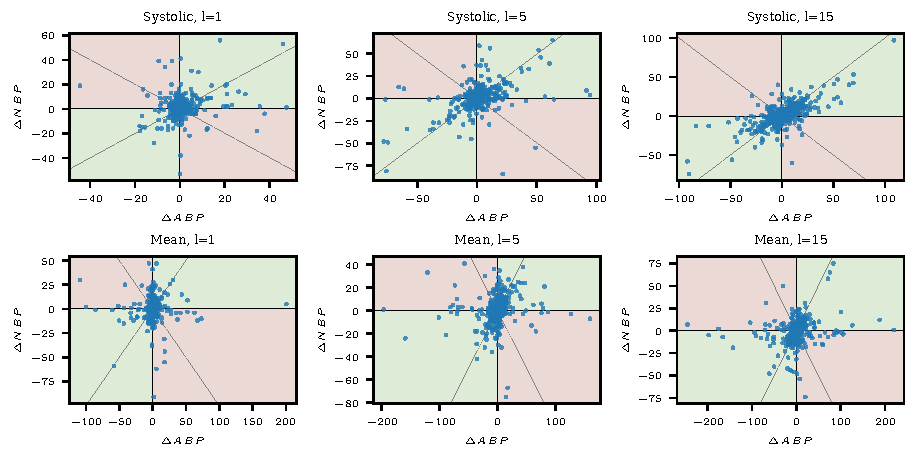
\includegraphics{plots/mimic/plot_4q}
    \caption{Four-quadrant plots for the different lags and the systolic and mean blood pressure measurements. The upper row contains systolic measurements and the lower row mean measurements. The columns contain the lags one, five, and 15 minutes.}
    \label{fig:app-mimic-4q}
\end{figure}

\begin{table}
    \centering
    \begin{tabular}{l l p{0.2\textwidth} p{0.2\textwidth} p{0.2\textwidth}}
\toprule
Type & $l$ & $\mu^{l}$ & $\mu^{+, l}$ & $\mu^{-, l}$ \\
\midrule
Systolic & 1 & {0.55 (0.50, 0.60)} & {0.59 (0.52, 0.65)} & {0.58 (0.50, 0.66)} \\
Systolic & 5 & {0.63 (0.59, 0.68)} & {0.70 (0.64, 0.75)} & {0.62 (0.56, 0.69)} \\
Systolic & 15 & {0.69 (0.65, 0.73)} & {0.72 (0.66, 0.76)} & {0.74 (0.69, 0.79)} \\
Mean & 1 & {0.55 (0.51, 0.59)} & {0.62 (0.56, 0.68)} & {0.56 (0.50, 0.62)} \\
Mean & 5 & {0.59 (0.55, 0.64)} & {0.65 (0.59, 0.71)} & {0.62 (0.56, 0.68)} \\
Mean & 15 & {0.62 (0.58, 0.65)} & {0.65 (0.60, 0.70)} & {0.66 (0.61, 0.71)} \\
\bottomrule
\end{tabular}

    \caption{Trending ratios for the different lags and the systolic and mean blood pressure measurements.}
    \label{tab:app-mimic-trending-ratios}
\end{table}

\begin{figure}
    \centering
    \begin{subfigure}[t]{.32\textwidth}
        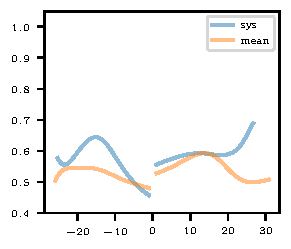
\includegraphics{plots/mimic/cond_prob_diff_nbp_abp_lag1}
        \caption{Lag one minute.}
    \end{subfigure}\hspace{0.01\textwidth}
    \begin{subfigure}[t]{.32\textwidth}
        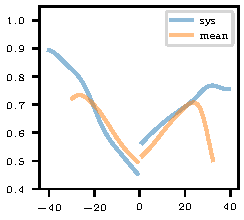
\includegraphics{plots/mimic/cond_prob_diff_nbp_abp_lag5}
        \caption{Lag five minutes.}
    \end{subfigure}\hspace{0.01\textwidth}
    \begin{subfigure}[t]{.32\textwidth}
        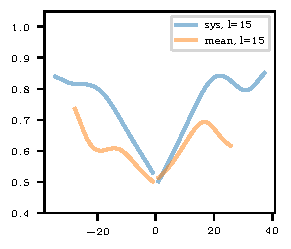
\includegraphics{plots/mimic/cond_prob_diff_nbp_abp_lag15}
        \caption{Lag 15 minutes.}
    \end{subfigure}\hspace{0.01\textwidth}
    \caption{Conditional trending plot for the systolic and mean blood pressure measurements and the lags one, five, and 15 minutes. \hl{Short interpretation.}}
    \label{fig:app-mimic-cond-prob}
\end{figure}




\subsubsection*{Discussion}

The four-quadrant plots contain a considerable number of extreme points.
It is not clearly distinguishable whether these points are due to measurement errors or actual extreme values.
Some authors argue to exclude not only the measurements below the 10\%-quantile of the absolute differences but also the points above the 90\%-quantile.
We do not follow this approach here, as the extreme values are not necessarily measurement errors and could also be particularly relevant.

The differences between positive and negative predicted changes are small in this example.
The positive and negative trending ratios have overlapping confidence intervals, and the conditional trending plots do not contain prominent deviations in the course.
This is in line with the four-quadrant plots, where no clear asymmetry is visible.

The bootstrap confidence intervals are wide.
For the trending ratio, the width is around 0.1, while it gets up to 0.16 for the negative trending ratio for systolic measurement and the lag of 1 minute.

